% Created 2015-07-26 Dom 21:02
\documentclass[11pt]{article}
\usepackage[utf8]{inputenc}
\usepackage[T1]{fontenc}
\usepackage{fixltx2e}
\usepackage{graphicx}
\usepackage{longtable}
\usepackage{float}
\usepackage{wrapfig}
\usepackage{rotating}
\usepackage[normalem]{ulem}
\usepackage{amsmath}
\usepackage{textcomp}
\usepackage{marvosym}
\usepackage{wasysym}
\usepackage{amssymb}
\usepackage{hyperref}
\tolerance=1000
\usepackage{minted}
\usemintedstyle{perldoc}
\newcommand{\tu}{\textunderscore}
\author{Alice Duarte Scarpa}
\date{2015-07-28}
\title{Proposta de Trabalho de Visualização da Informação}
\hypersetup{
  pdfkeywords={},
  pdfsubject={},
  pdfcreator={Emacs 24.4.1 (Org mode 8.2.10)}}
\begin{document}

\maketitle

\section{Introdução}
\label{sec-1}

O \href{https://www.mozilla.org/en-US/firefox/new/}{Firefox} é um projeto Open Source com muitos colaboradores. Toda vez
que um colaborador faz alguma modificação no projeto, cerca de 800
\href{https://treeherder.mozilla.org/#/jobs?repo=mozilla-inbound}{suítes de testes} rodam para garantir que o Firefox continua
funcionando depois de cada mudança. Idealmente, uma mudança só poderia
entrar no Firefox se passasse em todos os testes automatizados. Mas o
time de automação enfrenta um grande problema: Alguns testes falham
aleatoriamente.

Para lidar melhor com essa situação, o time de automação da Mozilla
começou o projeto \href{http://brasstacks.mozilla.com/orangefactor/}{OrangeFactor} que agrega dados sobres os testes
\emph{intermitentes}.

Meu objetivo nesse trabalho é criar visualizações que ajudem a
explorar os dados do OrangeFactor.

\section{Dados}
\label{sec-2}

\href{http://activedata.allizom.org/tools/query.html}{ActiveData} é uma ferramenta que permite criar consultas a vários dados
da automação Mozilla usando a \href{https://github.com/klahnakoski/ActiveData/blob/dev/docs/Qb_Expressions.md}{linguagem Qb}. A tabela abaixo é uma
amostra dos resultados depois de limpos:

\begin{center}
\begin{tabular}{llll}
revision & buildername & timestamp & bug\\
2efc03ac92f9 & MacOSX 10.8 opt mochitest-gl & 1420242226 & 1099173\\
47683fccda29 & Windows 8 64-bity debug mochitest-browser-chrome-1 & 1420237516 & 1013239\\
2efc03ac92f9 & Android armv7 API 9 opt mochitest-5 & 1420237489 & 1109932\\
2fbdaa8a5ea7 & Android 4.0 armv7 API 10+ opt robocop-3 & 1420240312 & 913870\\
2a7cd513b565 & b2g\tu emulator\tu vm debug mochitest-debug-3 & 1420240404 & 906716\\
2fbdaa8a5ea7 & Ubuntu VM 12.04 x64 debug mochitest-3 & 1420242170 & 1114682\\
9689b122bc76 & b2g\tu emulator\tu vm opt mochitest-6 & 1420237668 & 989048\\
8fcced3ba6d8 & MacOSX 10.6 debug mochitest-browser-chrome-1 & 1420247528 & 1015617\\
f22e7b280329 & Android armv7 API 9 opt mochitest-7 & 1420242967 & 1109932\\
9689b122bc76 & Android armv7 API 9 opt robocop-1 & 1420242375 & 851861\\
\end{tabular}
\end{center}

\section{Público alvo}
\label{sec-3}

A comunidade de automação da Mozilla.

\section{Ferramentas}
\label{sec-4}

\begin{itemize}
\item scripts em Python para manipular os dados
\item D3.js para gerar visualizações
\end{itemize}

\section{Objetivos}
\label{sec-5}

\begin{itemize}
\item Aprender a usar \href{http://d3js.org/}{D3.js}
\item Gerar visualizações utéis para a Mozilla
\end{itemize}

\section{Inspiração}
\label{sec-6}

Uma visualização que se encaixaria bem nesse contexto é um heatmap
mostrando quantos testes falharam por commit, baseado no gráfico que
aparece na página inicial do GitHub.

\href{http://github.com/adusca}{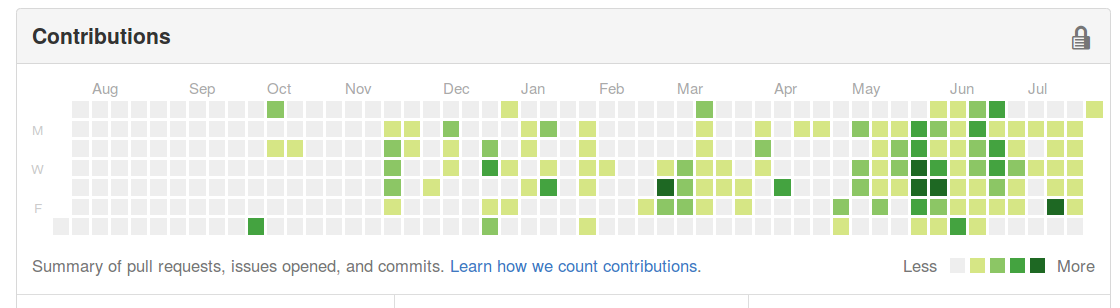
\includegraphics[width=.9\linewidth]{github-heatmap.png}}
% Emacs 24.4.1 (Org mode 8.2.10)
\end{document}
